\documentclass[12pt]{article}
\usepackage{fontspec}
\usepackage[utf8]{inputenc}
\setmainfont{Bodoni 72 Book}
\usepackage[paperwidth=17in,paperheight=11in,margin=1in,headheight=0.0in,footskip=0.5in,includehead,includefoot,portrait]{geometry}
\usepackage[absolute]{textpos}
\usepackage{xcolor}
\usepackage{background}
\usepackage{contour}
\TPGrid[0.5in, 0.25in]{23}{24}
\parindent=0pt
\parskip=12pt
\usepackage{nopageno}
\usepackage{graphicx}
\graphicspath{ {./images/} }
\usepackage{amsmath}
\usepackage{tikz}
\newcommand*\circled[1]{\tikz[baseline=(char.base)]{
            \node[shape=circle,draw,inner sep=1pt] (char) {#1};}}

\begin{document}

\backgroundsetup{scale = 1.075, angle = 0, opacity = 0.2,
contents = {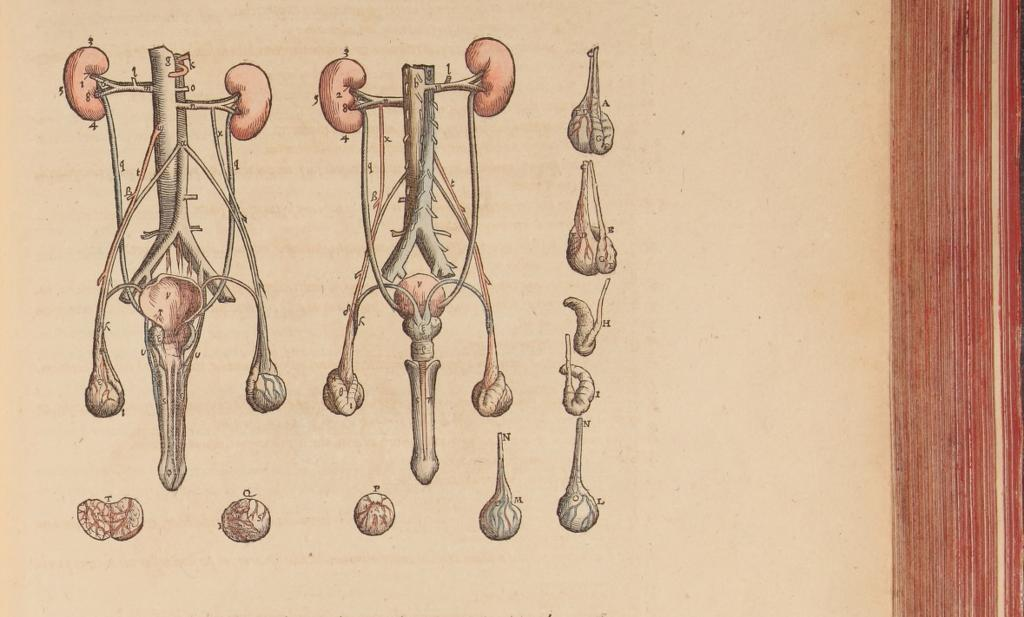
\includegraphics[width = \paperwidth,
height = \paperheight, keepaspectratio] {foreword_image.jpeg}}}

\vspace*{4.5\baselineskip}

\contourlength{0.04em}

\begingroup
\begin{center}
\fontsize{1.5cm}{1em} \selectfont{
\contour{white}{FOREWORD}
}
\end{center}
\endgroup

\vspace*{1\baselineskip}

\contourlength{0.07em}

\begingroup
\begin{center}
\fontsize{0.5cm}{1em} \selectfont{
{\setmainfont{Source Han Serif SC}\selectfont
\contour{white}{
``欲得长生,肠中当清;欲得不死,肠中无滓 . . .} \\
}
}
\end{center}
\endgroup

\begingroup
\begin{center}
\fontsize{0.5cm}{1em} \selectfont{
{\setmainfont{Source Han Serif SC}\selectfont
\contour{white}{
``一人之身,一国之象也。} \\
\contour{white}{
``胸腹之设,犹宫室也。肢体之位,犹郊境也。} \\
\contour{white}{
``骨节之分,犹百官也。腠理之间,犹四衢也。} \\
\contour{white}{
``神犹君也,血犹臣也,气犹民也,故治人能治其身,亦如明主能治其国 . . .} \\
\contour{white}{
``若能审机权,可以制嗜欲,保金性命。"} \\
\contour{white}{
- 葛洪}
}
}
\end{center}
\endgroup

\begingroup
\begin{center}
%\fontsize{0.5cm}{1em}
\contour{white}{
``Adorned with oxtails and plumes, they follow the rhythm of the chime stones and pitch pipes.} \\
\contour{white}{
In their purity and brilliance, they model themselves after Heaven.} \\
\contour{white}{
In their greatness and vastness, they model themselves after Earth.} \\
\contour{white}{
In their posturing and movements, they model themselves after the Four Seasons.} \\
\contour{white}{
Thus, when music is performed, their intentions become pure, and when ritual is cultivated their conduct is perfected.} \\
\contour{white}{
Their hearing becomes acute and their vision clear, the flowing of his blood and \textit{qi} harmonious and uniform, their practices altered, and their customs changed."} \\
\contour{white}{
- Burton Watson}
\end{center}
\endgroup

\end{document}